\section{Nichtlinearität (NL)}

\subsection{Umgang mit Nichtlinearität und Zeitvarianz}{84}

\begin{minipage}[c]{0.44\columnwidth}
	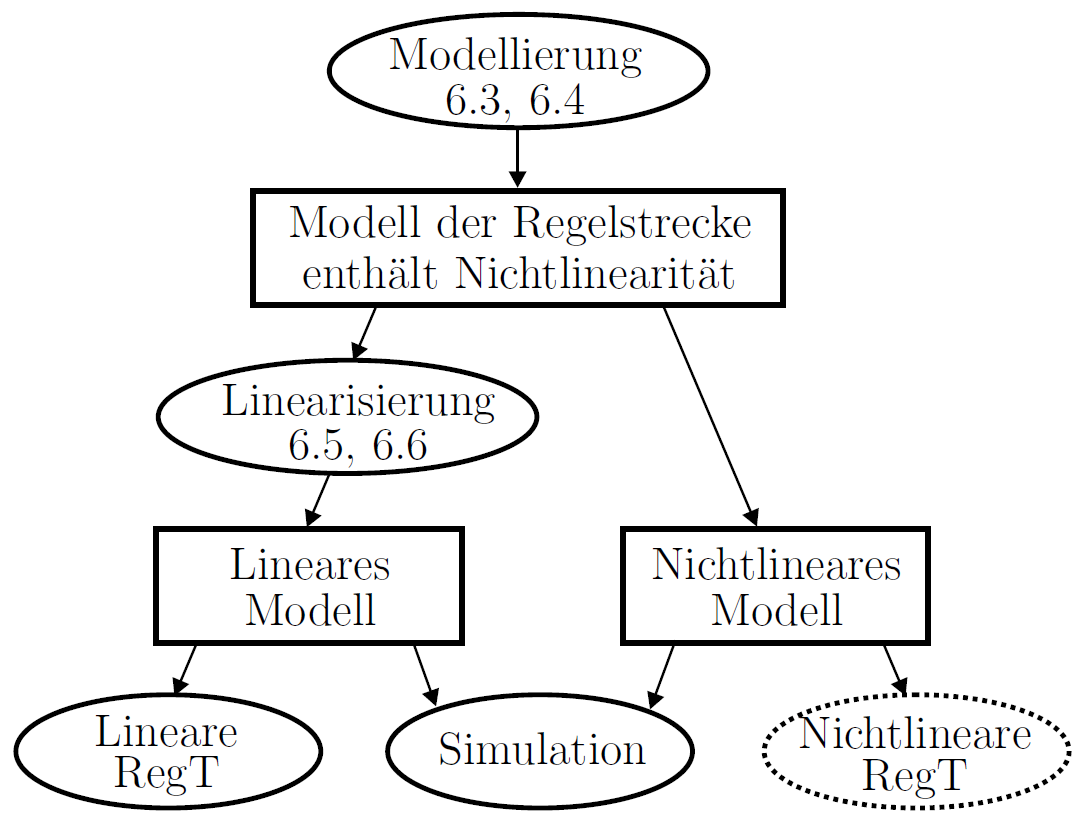
\includegraphics[width=\columnwidth]{images/vorgehen_nichtlineares_streckenmodell.png}
\end{minipage}
\hfill
\begin{minipage}[c]{0.48\columnwidth}
	\raggedright
	Für die Regler-Auslegungmöchten wir \textbf{lineare Systeme}.

	\vspace{0.2cm}

	Reale Systeme sind aber nichtlinear und zeitvariant
	\vspace{0.1cm}

	\begin{outline}
		\1 Sättigungen
		\1 Kennlinien
		\1 Physik
			\2 $F = k \cdot \cbl{i^2}$
			\2 $F = m \cdot g \cdot \cbl{\sin(\varphi)}$ 
	\end{outline}
\end{minipage}


\subsection{Modelle von Nichtlinearitäten (NL)}

Es gibt zwei Modelle, um Nichtlinearität darzustellen:

\vspace{0.2cm}

\begin{minipage}[t]{0.48\columnwidth}
	\textbf{Hammerstein-Modell} 
	\begin{center}
		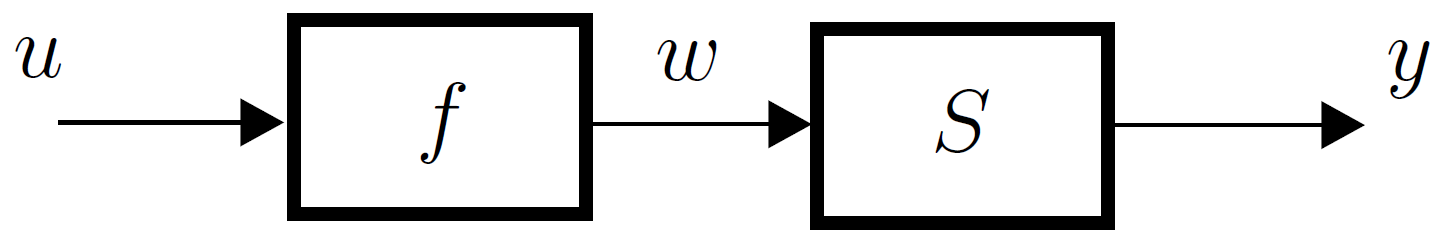
\includegraphics[width=0.9\columnwidth]{images/hammerstein.png}
	\end{center}
\end{minipage} 
\hfill
\begin{minipage}[t]{0.48\columnwidth}
	\textbf{Wiener-Modell} 
	\begin{center}
		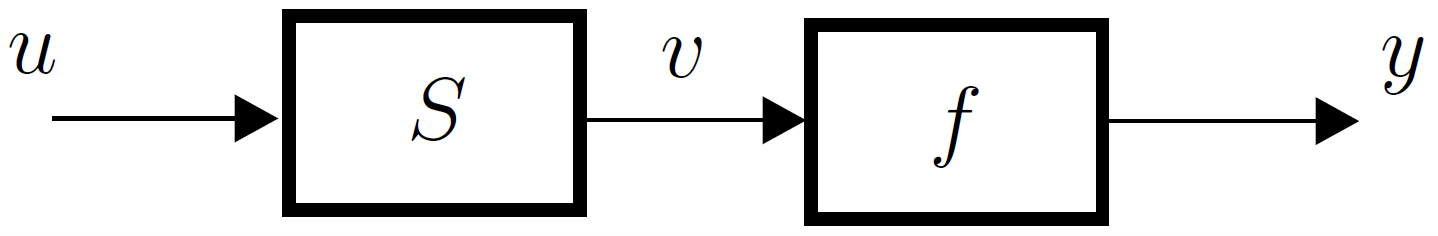
\includegraphics[width=0.9\columnwidth]{images/wiener.png}
	\end{center}
\end{minipage} 

\vspace{0.2cm}

\begin{tabular}{ll}
	$f$ & Nichtlinearität (z.B. Totzeit) 						\\
	$S$ & Stabiles (dynamisches) LZI-System mit Verstärkung 1
\end{tabular}


\subsection[Messung der statischen Kennlinie]{Messung der statischen Kennlinie von $\bm{f}$}{86}

Sowohl für das Hammerstein- als auch für das Wiener-Modell gilt: 
$$ y_{\rm stat} = f(u_{\rm stat}) \qquad \text{(eingeschwungener Zustand)} $$


\subsubsection{Vorgehen statische Messung der einzelnen Punkte}

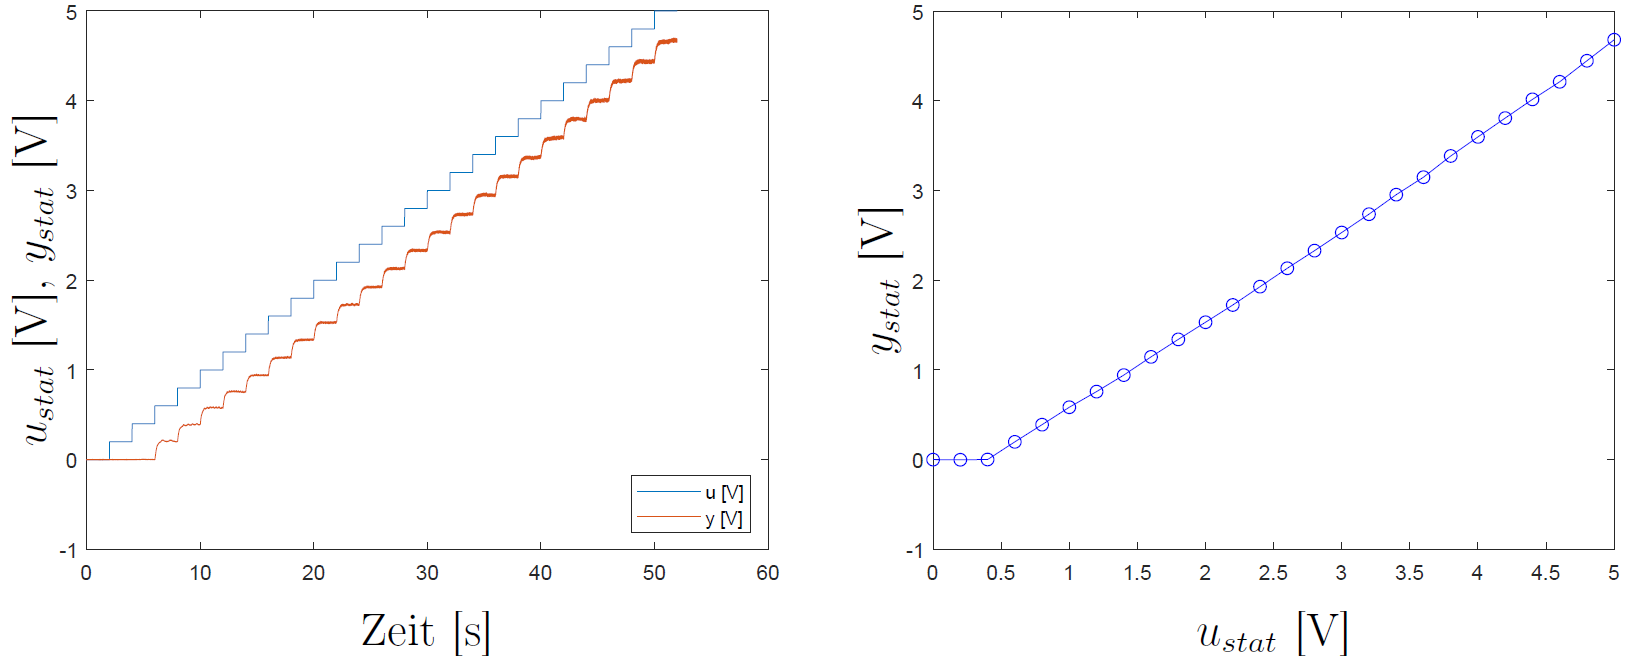
\includegraphics[width=\columnwidth]{images/messung_statische_kennlinie.png}

\begin{itemize}
	\item Eingang $u(t)$ \textbf{schrittweise} ändern (auf neuen Wert $u_{\rm stat}$) Augang $y(t)$ verändert sich stetig und schwingt 
		auf neuen Wert $y_{\rm stat}$ ein (überlagertes Rauschen)
	\item $y_{\rm stat}$ messen (z.B. durch Mittelwertbildung)
	\item Wertepaare $u_{\rm stat}, \, y_{\rm stat}$ ergeben Messpunkte $P_j = (u_j | y_j)$ der Kennlinie
	\item Annahmen über Kennlinie (Totzone, symm. bzgl. Nullpunkt) mit zusätzlichen Messpunkte
		(hier: $u_{\rm stat} > 5 \, V$ bzw. $u_{\rm stat} < 0 \, V$) absichern
\end{itemize}


\subsubsection{Vorgehen dynamische Messung}

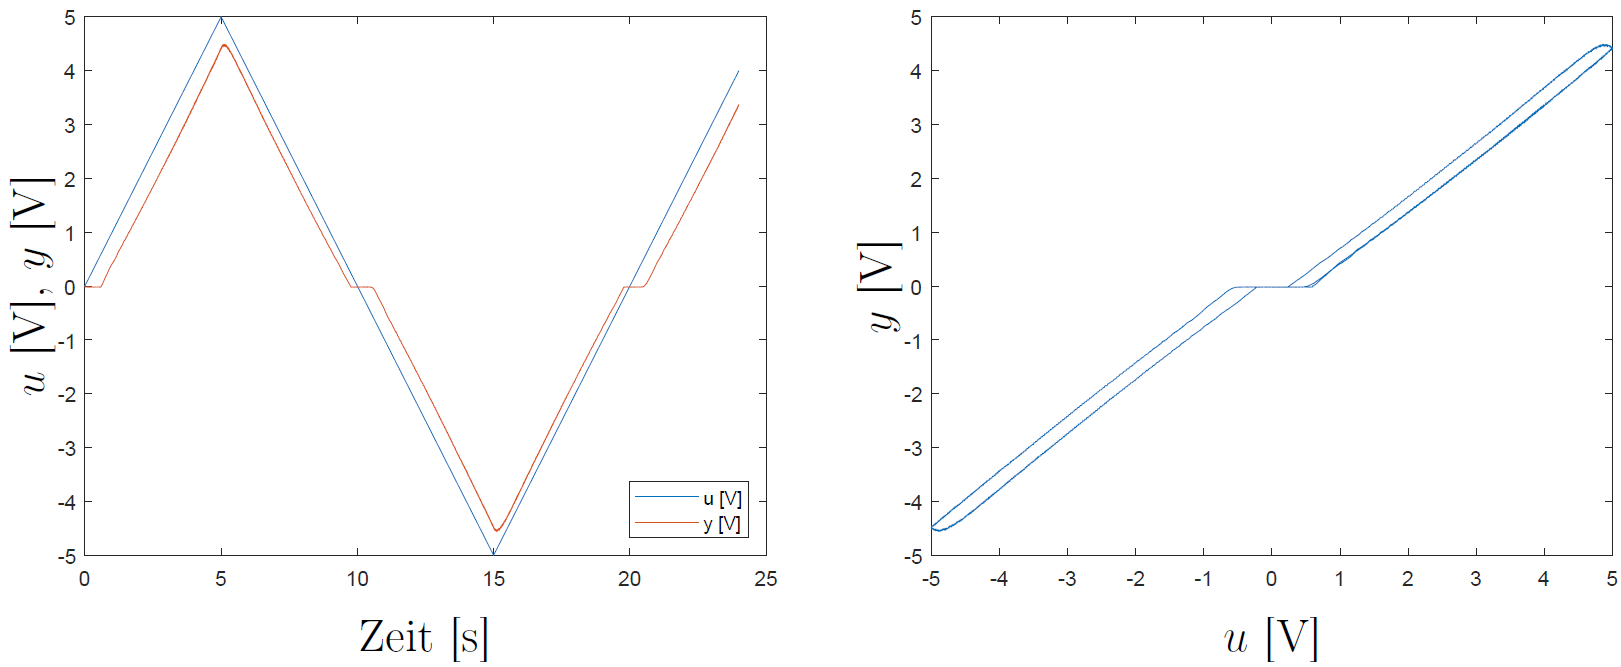
\includegraphics[width=\columnwidth]{images/dynamische_messung_kennlinie.png}

\begin{itemize}
	\item Eingang $u(t)$ \textbf{kontinuierlich} ändern (rampenförmig) \\
		Ausgang $y(t)$ schwingt nicht ein, sondern läuft stationärem Wert stets hinterher \\
		\textrightarrow\ Es entsteht eine \textbf{Pseudohysterese}
	\item Pseudohystere erkennen: Messgeschwindigkeit variieren \\
		\textrightarrow\ $N$ mal langsamere Messung \textrightarrow\ $N$ mal schmalere Hysterese
\end{itemize}


\subsection{Erfassung der NL -- Tabelle}

Die Messung der statischen Kennlinie von $f$ liefert Messpunkte $P_j = (u_j | y_j)$ mit $j = 1 \, ... \, N$ \\
Im einfachsten Fall werden diese Messpunkte als \textbf{Lookup-Table (LUT)} gespeichert.

\vspace{0.2cm}

Diese Form der Datenerfassung kann vor allem bei \textbf{vektoriellen Eingängen} (mehrere Eingangssignale) problematisch werden (Speicherplatz)


\subsection[Erfassung der NL -- Funktion]{Erfassung der NL -- Funktion $\bm{y = f(u)}$}

Eine Kennlinie stellt eine kompaktere Form der Datenerfassung dar. \\
Die Motivation kann auch darin liegen, dass Kennlinien einen \textbf{bekannten physikalischen Effekt} repräsentieren und es nun darum geht,
\textbf{einen oder mehrere Parameter} zu bestimmen.

\vspace{0.2cm}

\textbf{Gesucht wird also eine \textbf{gut passende Funktion} $y = f(u)$}

\vspace{0.1cm}

\begin{itemize}
	\item Idealerweise $y_j = f(u_j) \, \forall j$
	\item Struktur von $f$ beruht auf physikalischem Vorwissen oder möglichst einfache Struktur von $f$
\end{itemize}


\subsubsection{Gleichungssysteme ohne Lösungen}

Hat ein Gleichungssystem keine Lösung (überbestimmt), so führt man einen Fehlerterm $\varepsilon$ in die Gleichung ein:
$$ y_i = f(u_i) = \sum\limits_{i=1}^M \theta_i \cdot f_i(u_j) + \varepsilon_j $$
Nun kann eine Lösung für $\theta$ gesucht werden, bei der dieser Fehler möglichst klein werden (\textbf{\textrightarrow\ Least Squares}) \\
Beispielsweise wird dabei die Zielfunktion $J(\varepsilon) =  \sum\limits_{i=1}^M \varepsilon_i^2$ minimiert.


\subsubsection{Funktion linear in Parametern (l.i.p.)}

Eine Funktion $f$ ist l.i.p. , falls sie die folgenden Form hat.
$$ y = f(u) = \theta_1 \cdot f_1(u) + \theta_2 \cdot f_2(u) + ... = \sum\limits_{i=1}^M \theta_i \cdot f_i(u_j) $$ 
Die Werte $\theta_i$ sind dabei die unbekannten Parameter.


\example{l.i.p. Gleichungssystem mit eindeutiger Lösung}

\vspace{-0.2cm}

$$ \text{Ansatz:} \quad  \cgn{y} = f(u) = \theta_1 \cdot \cbl{u} + \theta_2 \cdot \cor{u^2} \text{ mit 2 Messpunkten } (\cbl{u_j} \, | \, \cgn{y_j}) $$
$$ \begin{vmatrix} \cgn{1.0} = \theta_1 \cdot \cbl{0.8} + \theta_2 \cdot \cor{0.64} \\ \cgn{2.0} = \theta_1 \cdot \cbl{3.0} + \theta_2 \cdot \cor{9.0} \end{vmatrix}
\text{ \textrightarrow\ } \underbrace{ \begin{bmatrix} \cgn{1.0} \\ \cgn{2.0} \end{bmatrix} }_{\substack{y}} = \underbrace{ 
\begin{bmatrix} \cbl{0.8} & \cor{0.64} \\ \cbl{3.0} & \cor{9.0} \end{bmatrix} }_{\substack{\Phi}} \, \underbrace{\begin{bmatrix}  \theta_1 \\ \theta_2 \end{bmatrix} }_{\substack{\theta}}$$
$$ \theta = \Phi^{-1} \cdot y = \underbrace{  \frac{1}{0.8 \cdot 9.0 - 3.0 \cdot 0.64} \begin{bmatrix} 9.0 & -0.64 \\ -3.0 & 0.8 \end{bmatrix} }_{\substack{\Phi^{-1}}}
\, \begin{bmatrix} 1.0 \\ 2.0 \end{bmatrix} = \begin{bmatrix} 1.46 \\ -0.27 \end{bmatrix}$$


\example{l.i.p. überbestimmtes Gleichungssystem}

\vspace{-0.2cm}

$$ \text{Ansatz:} \quad \cgn{y} = f(u) = \theta_1 \cdot \cbl{u} + \theta_2 \cdot \cor{u^2} \text{ mit 3 Messpunkten } (\cbl{u_j} \, | \, \cgn{y_j}) $$
$$ \begin{vmatrix} \cgn{1.0} = \theta_1 \cdot \cbl{0.8} + \theta_2 \cdot \cor{0.64} \\  \cgn{2.5} = \theta_1 \cdot \cbl{2.0} + \theta_2 \cdot \cor{4.0} \\ 
\cgn{2.0} = \theta_1 \cdot \cbl{3.0} + \theta_2 \cdot \cor{9.0} \end{vmatrix} \text{ \textrightarrow\ } 
\underbrace{ \begin{bmatrix} \cgn{1.0} \\ \cgn{2.5} \\ \cgn{2.0} \end{bmatrix} }_{\substack{y}} = 
\underbrace{ \begin{bmatrix}  \cbl{0.8} & \cor{0.64} \\ \cbl{2.0} & \cor{4.0} \\ \cbl{3.0} & \cor{9.0} \end{bmatrix} }_{\substack{\Phi}} \,
\underbrace{\begin{bmatrix}  \theta_1 \\ \theta_2 \end{bmatrix} }_{\substack{\theta}}$$
$$ \boxed{ \theta_{\rm opt} = \underbrace{ (\Phi^T \Phi)^{-1} \Phi^T }_{\substack{P}} \cdot y  \quad \text{(Least Squares)} } $$


\myul{\textbf{Moore-Penrose'sche Pseusodinverse $P$ in Matlab:}}
%DONE: listings
\mylstbox{theta = phi \\ y}
% \textbf{Matlab:} $\boldsymbol{\theta = \Phi \backslash y}$


\subsubsection{Funktion nichtlinear in Parametern (nicht l.i.p.)}

\example{Nicht l.i.p. Gleichungssystem mit mehreren Lösungen}

\vspace{-0.2cm}
$$ \text{Ansatz:} \quad \cgn{y} = f(u) = \theta_1 \cdot \sin( \theta_2 \cdot \cbl{u}) \text{ mit 2 Messpunkten } (\cbl{u_j} \, | \, \cgn{y_j}) $$ 
$$ \begin{vmatrix} \cgn{1.0} = \theta_1 \cdot \sin(\cbl{0.8} \cdot \theta_2 ) \\  \cgn{2.0} = \theta_1 \cdot \sin(\cbl{3.0}  \cdot \theta_2 ) \end{vmatrix} 
\text{ \textrightarrow\ } \frac{ (\Romannum{1}) }{(\Romannum{2}) } \text{ \textrightarrow\ }
0.5 = \frac{\sin(\cbl{0.8} \cdot \theta_2)}{\sin(\cbl{3.0}  \cdot \theta_2 )} $$

Sinus-Term plotten und mehrere Schnittpunkte (Lösungen) finden


\example{Nicht l.i.p. Gleichungssystem}

\vspace{-0.2cm}
$$ \text{Ansatz:} \quad \cgn{y} = f(u) = \theta_1 \cdot \sin( \theta_2 \cdot \cbl{u}) \text{ mit 3 Messpunkten } (\cbl{u_j} \, | \, \cgn{y_j}) $$
$$ \begin{vmatrix} \cgn{1.0} = \theta_1 \cdot \sin(\cbl{0.8} \cdot \theta_2 ) + \varepsilon_1 \\ \cgn{2.5} 
= \theta_1 \cdot \sin(\cbl{2.0}  \cdot \theta_2 )  + \varepsilon_2  \\ \cgn{2.0} 
= \theta_1 \cdot \sin(\cbl{3.0}  \cdot \theta_3 )  + \varepsilon_2\end{vmatrix}  \text{ \textrightarrow\ Fehler minimieren} $$

Es entstehen differentielle Ableitungen mit vielen Sinus-Termen, welche Null gesetzt werden müssen \textrightarrow\ mühsam!

\vspace{0.2cm}
\textbf{Man verwendet besser ein lineares Modell, dann gibt es auch nur eine Lösung!}


\subsection{Linearisierung durch Veränderung der Strecke}

\subsubsection{Inversion der Kennlinie}

Um die Nichtlinearität $f$ in der Strecke zu kompensieren wird am Ausgang des Reglers die 
\textbf{Umkehrfunktion der Nichtlinearität} $f^{-1}$ eingefügt.\\
Somit wird $w = \tilde{u}$ und der Regler hat nur das $\text{PT}_1$-Glied als Regelstrecke 

\begin{center}
	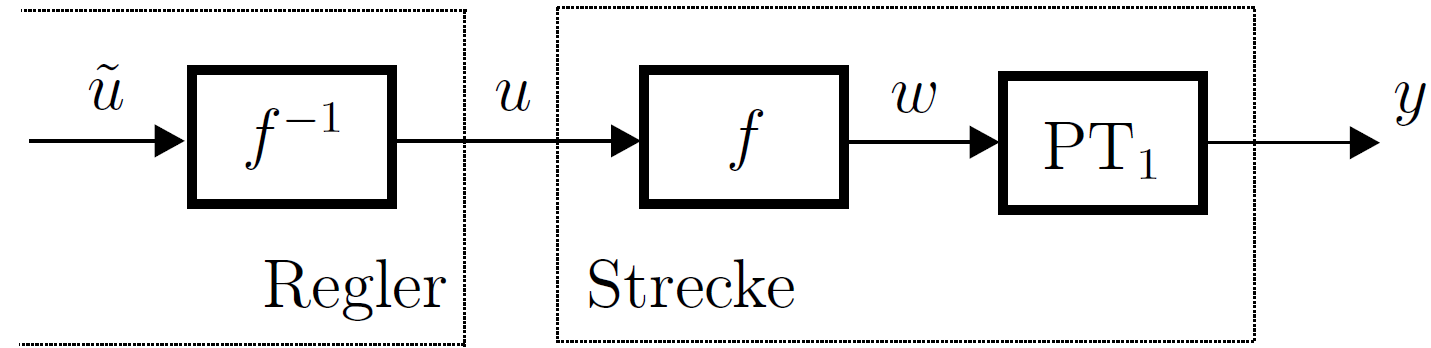
\includegraphics[width=0.7\columnwidth]{images/linearisierung_inversion_kennlinie.png}
\end{center}


Egal wo die Nichtlinearität ist, es muss am 'passenden Ort' im Blockdiagramm die \textbf{Umkehrfunktion der Nichtlinearität} eingefügt werden. \\
\textrightarrow\ ggf. Verschiebungsregeln aus Kapitel ~\ref{Serieschaltung von LZI-Systemen} anwenden 

\vspace{0.2cm}

\textbf{Bemerkungen} 
\vspace{0.1cm}

\begin{itemize}
	\item $f$ kann nicht in allen Fällen invertiert werden \\
		 \textrightarrow\ Sättigungen am Streckeneingang besitzt kein $f^{-1}$ 
	\item Es muss nicht zwischen Wiener- und Hammersein-Struktur unterschieden werden\\
		\textrightarrow\ Gleiches Vorgehen 
\end{itemize}


\subsubsection{Gegenkopplung unterlagerte Regler}

Ein Regler hält den Fehler $e$ bei $0$. Schafft er das, dann ist $y(t) \approx r(t)$ und somit das Gesamtverhalten 'einigermassen' linear.

\begin{center}
	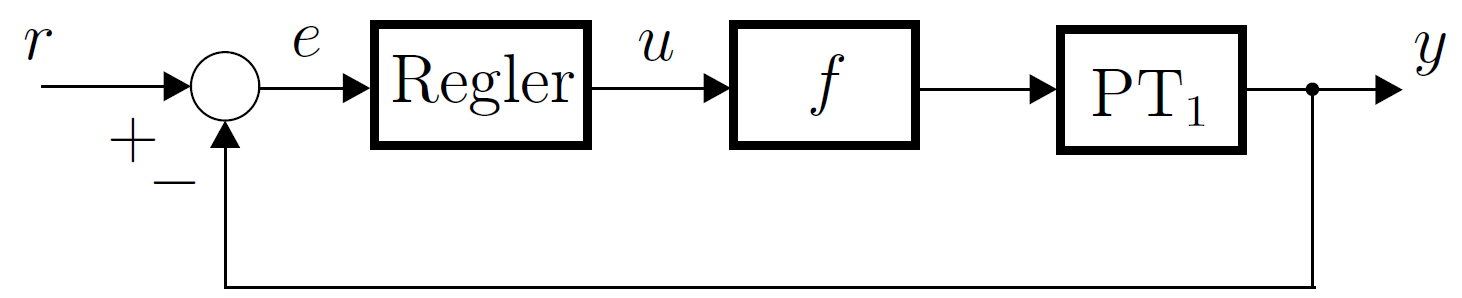
\includegraphics[width=0.7\columnwidth]{images/unterlagerte_regelung.png}
\end{center}


\begin{itemize}
	\item  Überlagerter Regler 'sieht' ein einfaches P-Glied mit $K = 1$ \\
		\textrightarrow\ \textbf{Unterlagerter (linearisierender) Regler} muss \textbf{schneller} sein als überlagerter Regler
		\item Kaskadenreglung 
\end{itemize}

\vspace{0.2cm}
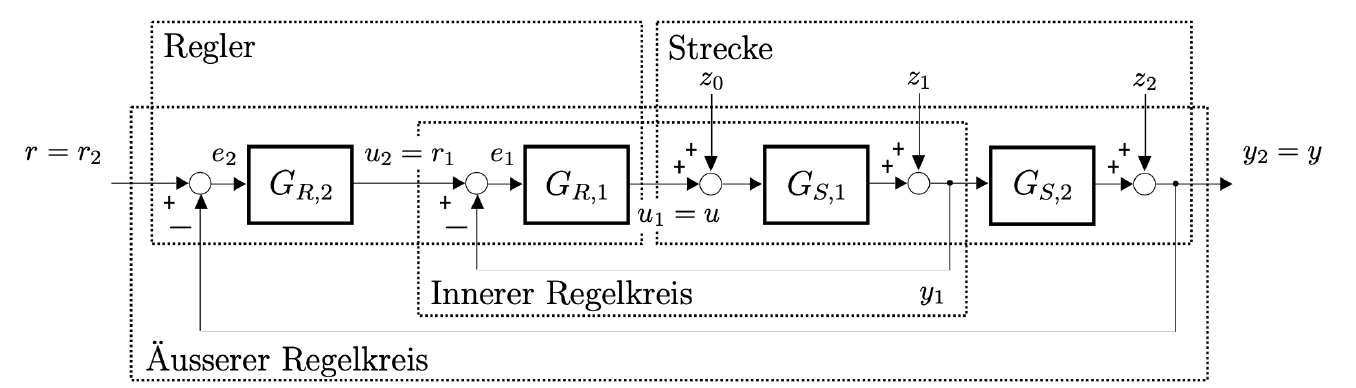
\includegraphics[width=\columnwidth]{images/kaskadenregelung}


\subsection{Linearisierung durch Vereinfachung}{94}

Idee: In einem Arbeitspunkt verhält sich das System 'genügend' linear\\
\textrightarrow\ konstanter Wert \textbf{(steady state)} 


\subsubsection{Steady State}

Ist ein System im 'Steady State', so gilt: 
\vspace{0.1cm}

\begin{minipage}[t]{0.48\columnwidth}
	\begin{itemize}
		\item Fehler $e(t) = 0 $
	\end{itemize}
\end{minipage}
\hfill
\begin{minipage}[t]{0.48\columnwidth}
	\begin{itemize}
		\item Ableitungen $= 0$ 
	\end{itemize}
\end{minipage}


\subsubsection{Vorgehen Linearisierung im Arbeitspunkt}

\begin{minipage}{0.48\columnwidth}
	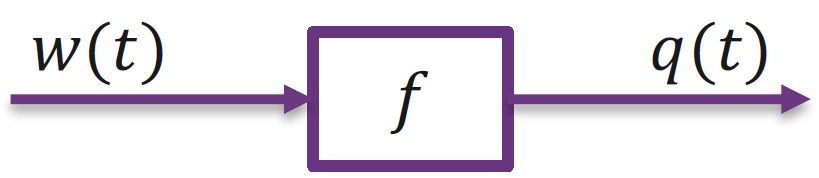
\includegraphics[width=0.7\columnwidth]{images/linearisierung_vereinfachung_1.png} 
\end{minipage}
\hfill
\begin{minipage}{0.48\columnwidth}
	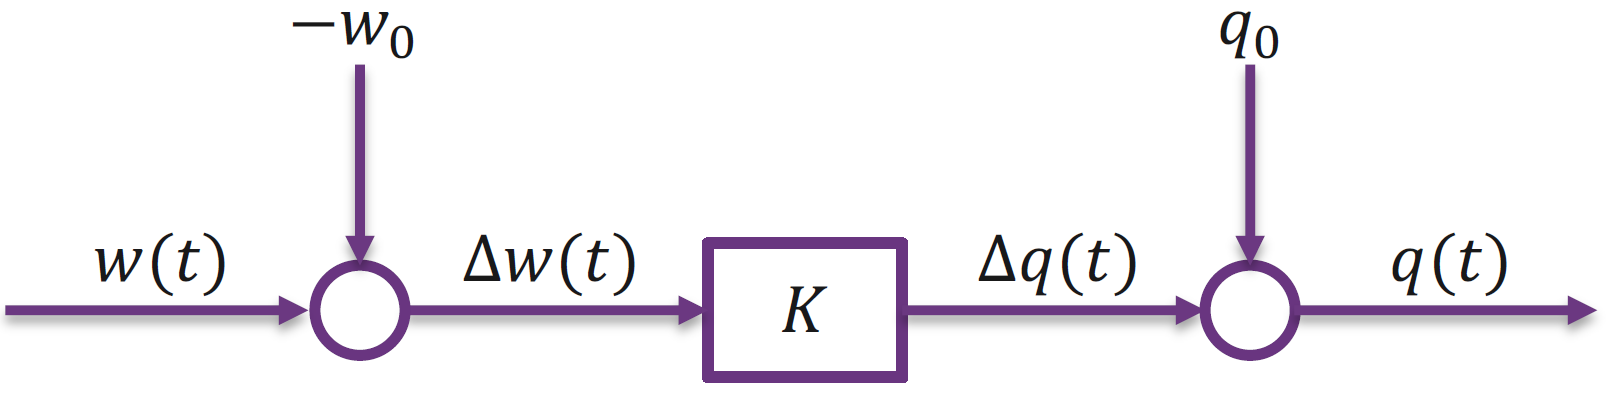
\includegraphics[width=\columnwidth]{images/linearisierung_vereinfachung_2.png} 
\end{minipage}

\vspace{0.2cm}

\begin{enumerate}
	\item Alle Signale durch $x(t) = x_0 + \Delta x(t)$ ersetzen \\
		(Nominalwerte $x_0 = \text{const}$ und kleine Abweichung $\Delta x(t)$)
	\item Nominalwert $x_0$ festlegen / bestimmen \\
		\textrightarrow\ Typischerweise der Sollwert $y_0$ für Regelgrösse $y$
	\item \cgn{Signale im Blockdiagramm durch $\Delta x(t)$ ersetzen}
	\item \cbl{Anpassung Eingang: $w(t) = \Delta w(t) - w_0$ (Subtraktion)} \\
		\crd{Anpassung Ausgang: $q(t) = q_0 + \Delta q$ (Addition)}
	\item Lineare Blöcke übernehmen
	\item \cor{Nichtlineare Blöcke durch Näherungen (z.B. Gain) ersetzen \textrightarrow\ \textbf{Steady-State} beachten} 
		\begin{itemize}
			\setlength\itemsep{0.75em}
			\item $q(t) = f(w(t)) \;$ \textrightarrow\ $\Delta q(t) = K \cdot \Delta w(t)$
			\item $K = \frac{\diff q}{\diff w} \Big|_{w=w_0}$ (Steigung im Arbeitspunkt) 
			\item $\bm{q(t) \approx q_0 + K \cdot \Delta w(t) = q_0 + K \cdot (w(t) - w_0)$} \quad \textrightarrow\ $\bm{q_0 = q(t_0)}$
		\end{itemize}
\end{enumerate}

   
\example{Linearisierung Auto}   
\begin{center}
	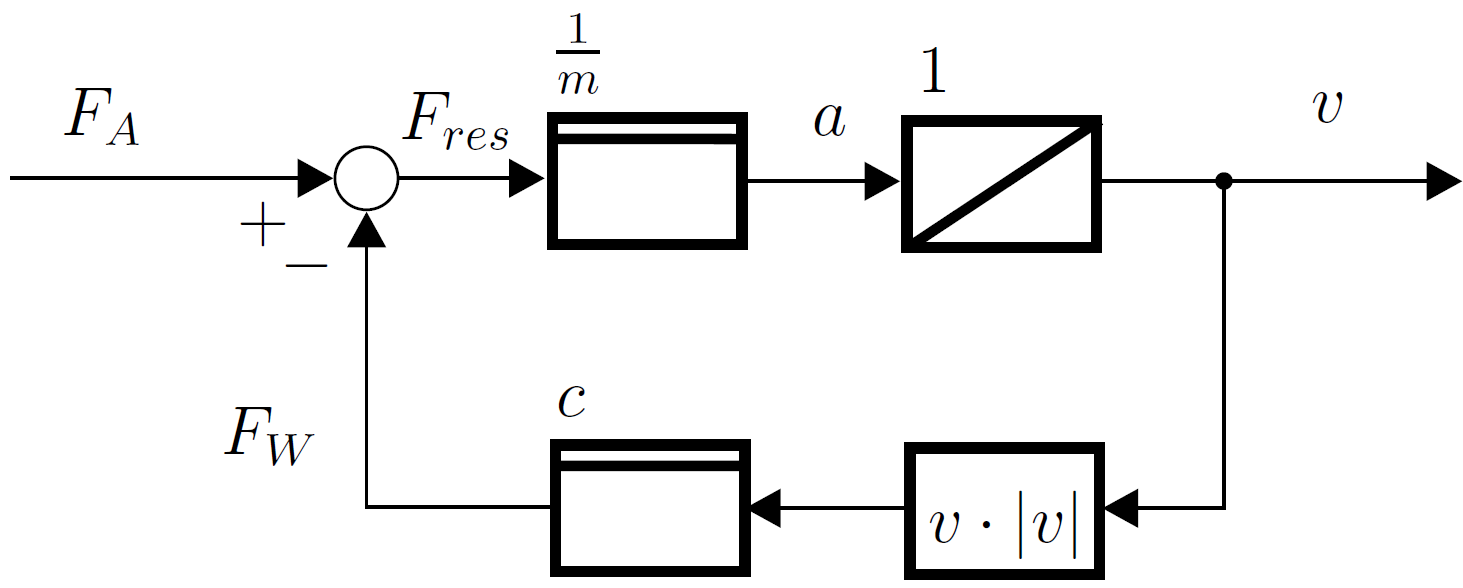
\includegraphics[width=0.6\columnwidth]{images/beispiel_linearisierung_1.png}
	\vspace{0.2cm}
	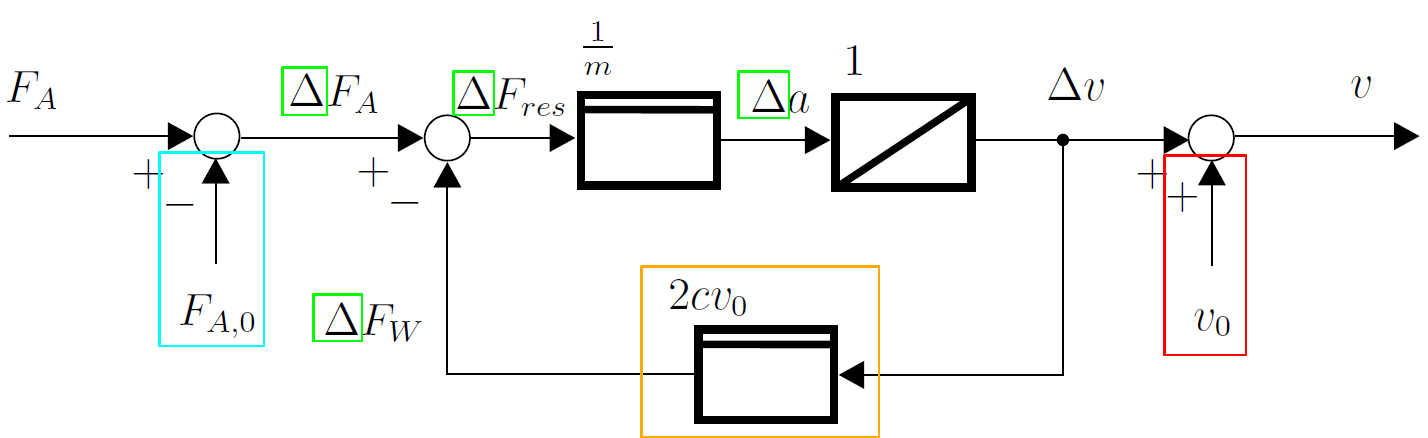
\includegraphics[width=0.8\columnwidth]{images/beispiel_linearisierung_2.png}
\end{center}

\vspace{-0.2cm}

\renewcommand{\arraystretch}{1.8}
\begin{tabular}{l}
	Nominalgeschwindigkeit: $v_0 > 0 = \const$ \\
	$v_0 = \const$ \quad \textrightarrow\ $a_0 = 0$ \quad \textrightarrow\ $F_{ \rm res, 0} = 0 $ \\
	$ F_{A,0} = F_{W,0}$ \quad \textrightarrow\ $F_{W,0} = c \cdot v_0^2$ \quad \textrightarrow\ $ F_{A,0} = c \cdot v_0^2$ 
\end{tabular}
\renewcommand{\arraystretch}{1}

\vspace{0.2cm}

\myul{\textbf{Rechenweg Linearisierung}}

\vspace{0.2cm}

\begin{minipage}[c]{0.34\columnwidth}
	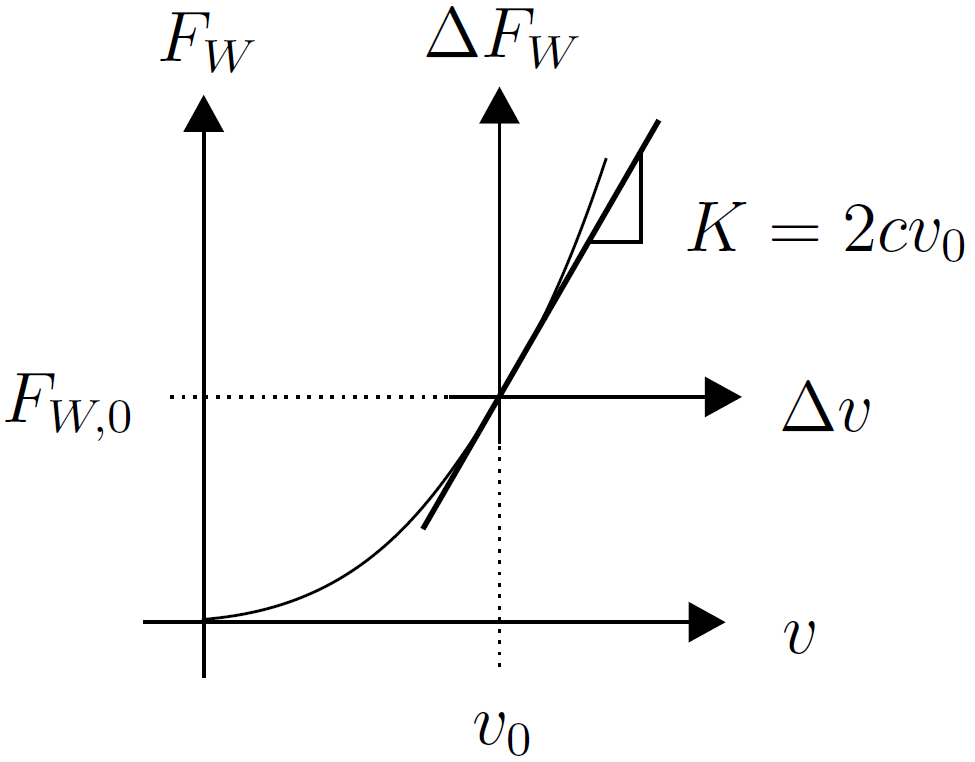
\includegraphics[width=\columnwidth]{images/beispiel_linearisierung_3.png} 
\end{minipage}
\hfill
\begin{minipage}[c]{0.58\columnwidth}
		$$ F_W = c \cdot v^2 $$
		$$ \frac{\diff F_W}{\diff v} \big| _{v = v_0} = c \cdot 2 \cdot v \big| _{v = v_0} = \underbrace{2 \, c \, v_0}_{K} $$
		$$ \Delta F_W \approx K \cdot \Delta v $$
\end{minipage}

